%\vspace{-0.15in}
\chapter{Model Generator}
\label{sec:model}

\section{Modeling an IoT system}
To correctly verify safety properties, we need to model two key components (not part of the app code):
(i) the IoT platform and its interactions with smart apps and
(ii) IoT devices and their interactions with smart apps.
{\color{black}IoT platforms~\cite{iftttpage,Samsung:smartthings,Apple:homekit,Amazon:alexa,Microsoft:iot} typically provide apps with some methods to register callback functions (\ie, event handlers).
Based on apps' configurations provided by the \textit{Configuration Extractor}, we model these special registration functions so as to invoke callbacks at appropriate times.}
\begin{comment}
With regards to the SmartThings platform, we first need to model its platform SDKs, which are unfortunately not open sourced.
Thus, we model the major classes and methods based on the SmartThings documentation~\cite{Samsung:smartthingsapi}.
The example classes include \textit{Command, Attribute, Event, Mode, State, and Location.}
%Each object (\textit{e.g.}, attribute, command, capability, state, event, and device) is modeled by a Groovy class.
%All of these classes are packaged into a library, which is automatically imported by \textit{GParser} when parsing smart apps' source files. \zhiyun{I think this is more related to modeling of the SmartThings framework and not so much about translator (so I moved it here)}
In addition, the SmartThings platform allows apps to register callback functions (\ie, event handlers)
via $subscribe$ and $schedule$ methods.
%Since we need the info of event handlers in analyzing app dependency and generating Promela model, we also extract this info in this phase.
We model these special registration functions so as to invoke callbacks at appropriate times.
\end{comment}


We model IoT devices (sensors and actuators) as per their specifications.
Note that both sensors and actuators can generate events of interest to apps.
For instance, a motion sensor can generate motion active/inactive events
whereas a door lock (actuator) can generate status update events (locked\allowbreak /unlocked).
%The difference is that actuators can take commands from apps (\eg, lock/unlock a door).
Each device is modeled as having an event queue
and a set of notifiers to inform the smart apps that have subscribed to specific types of events.
Currently, we support 30 different IoT devices.
%We use a global array to store all devices of same type in a system (\textit{e.g.}, $\_g\_STSwitchArr$ stores info of all switch devices in a system).
%A device assigns a specific slot in its subscriber notifiers to each subscriber. Whenever an event happens, a device will update its subscriber notifiers. A smart app will check its assigned slot in the subscriber notifiers of its subscribed device to see if any event happens. If the assigned slot is greater than $0$, the smart app will check the event queue to get the latest events, process them, and reset the slot to $0$. A smart app may send commands to some actuators via method call.
{\color{black} Note here that we model events generated by
the environment (\eg, $sunrise$ and $sunset$) as sensor generated inputs
and location mode changes 
(\textit{e.g.}, $Home$, $Away$, and $Night$) as actuations;
thus inputs such as users leaving home (sensed input) can trigger the mode to change from $Home$ to $Away$ (actuation).} 

{\color{black}We model system time as a monotonically
increasing variable. We extract the triggering times and callback functions from the scheduling
method calls. The callback functions are then triggered at appropriate times based on the value of
the modeled system time.}

\begin{comment}
{\color{black} Note here that we model the environment event (\eg, $sunrise$ and $sunset$) manager as a sensor device
and location mode 
(\textit{e.g.}, $Home$, $Away$, and $Night$) manager as an actuator,
which can take commands from some apps such as users leaving home and may trigger the mode to change from \textit{Home} to \textit{Away}.}
\end{comment}

Algorithm~\ref{alg:smarthingprocess} shows the pseudo code of the main process that models behaviors of an IoT system.
%\zhiyun{What is the ``SmartThings process''? It is the overall event simulation loop of the whole IoT system? Can we simplify the pseudo code? It is too long at the moment} \thomas{Yeah, it is the event simulation loop of the whole IoT system. I have simplified it. What do you think?}.
The model checker enumerates all possible permutations of the input physical events
up to a maximum number of events per user's configuration
to exhaustively verify the system.
At each iteration, a sensor and a corresponding physical event in the permutation space are selected (line 2).
Then, the selected sensor updates its state and event queue,
and notifies its subscribers of the state change event (line 3).
When an event is pending,
it is dispatched to the subscribed apps and the corresponding event handlers of apps are invoked to handle the event (lines 4-6).
Each event handler may send some commands to some actuators,
which may generate some new cyber events and trigger event handlers of the subscribers.

\begin{algorithm}[tb]
%\small
\ssp
\small
 \caption{Modeling an IoT system}
 \label{alg:smarthingprocess}
 \begin{algorithmic}[1]
 %\renewcommand{\algorithmicrequire}{\textbf{Input:}}
 %\renewcommand{\algorithmicensure}{\textbf{Output:}}
 %\REQUIRE None
 %\ENSURE  None
  %\COMMENT{\textbf{Main event loop of an IoT system}}
  \FOR[\textit{Main event loop of an IoT system}]{$i = 1$ to maximum number of events}
  \STATE Select a sensor and a corresponding event in the permutation space \COMMENT{\textit{Generate a physical event}}
  \STATE sensor\_state\_update(evt)
  \WHILE {any event pending}
  	\STATE dispatch\_event(evt) \COMMENT{\textit{Dispatch the pending event to the subscribed apps and invoke the corresponding app\_event\_handler(evt) to process the event}}
  \ENDWHILE
  \ENDFOR
  \\ \COMMENT{\textbf{sensor\_state\_update(evt)}}
  \IF {$evt \neq$ current state of the sensor}
 	\STATE Add the $evt$ to the event queue
 	\STATE Update the state of the sensor
 	\STATE Notify the subscribers of the state change event
 \ENDIF
  \\ \COMMENT{\textbf{app\_event\_handler(evt)}}
  \IF {some conditions hold}
 	\STATE Send some command to some actuator \COMMENT{\textit{Invoke actuator\_state\_update(evt), which may subsequently generate some new event}}
 \ENDIF
  \\ \COMMENT{\textbf{actuator\_state\_update(evt)}}
  \STATE Verify conflicting and repeated commands violations
  \IF {$evt \neq$ current state of the actuator}
 	\STATE Add the $evt$ to the event queue
 	\STATE Update the state of the actuator
 	\STATE Notify the subscribers of the state change event
 \ENDIF
 \end{algorithmic}
 \end{algorithm}



To model natural or induced (\textit{e.g.}, using jamming~\cite{5473884}) device/communication 
failures, 
when generating a sensor event we enumerate two scenarios:
(i) the sensor is available/online and (ii) the sensor is unavailable/offline.
Similarly, whenever receiving a command from a smart app,
an actuator may be either online or offline.
If a device is offline, it will not change its state and hence {\em not} broadcast a state change event to its subscribers. {\color{black}If a device is online, 
the communication (\ie, sending a state change event or receiving a command) between the device and the hub/cloud may either succeed or fail (we enumerate both cases).}

\begin{table}[tb]
\ssp
%\vspace{-0.16in}
\caption{Sample safe physical states.}
%\vspace{-0.12in}
\label{table:racescenarios}
\centering
{
{\color{black}\begin{tabular}{| p{1.9cm} | p{0.5cm} | p{11.5cm} |}
\hline
\bf Category & \bf \# & \bf Property\\
\hline
\multirow{5}{1.9cm}{Thermostat, AC, and Heater} & 1 & Temperature should be within a predefined range when people are at home\\ \cline{2-3}
 & 2 & An AC and a heater should not be both turned on\\ \cline{2-3}
 & 3 & The cooling set-point of a thermostat should be set to a value which is the same as the configured one\\ \cline{2-3}
 & 4 & The heating set-point of a thermostat should be set to a value which is the same as the configured one\\ \cline{2-3}
 & 5 & Thermostat should be turned off when a window/door is opened\\ \cline{2-3}
\hline
\multirow{8}{1.9cm}{Lock and door control} & 1 & The main door should be locked when no one is at home\\ \cline{2-3}
& 2 & The main door should be locked when people are sleeping\\ \cline{2-3}
& 3 & The main door should be locked when no one is at home and smoke detector state is clear\\ \cline{2-3}
& 4 & The main door lock should be locked when people are sleeping and smoke detector state is clear\\ \cline{2-3}
& 5 & A door control should be closed when no one is at home\\ \cline{2-3}
& 6 & When a door is closed, a lock should be locked\\ \cline{2-3}
& 7 & When all people leave home, some locks should be locked and location mode should be changed to Away\\ \cline{2-3}
& 8 & A door should be locked after being unlocked\\ \cline{2-3}
\hline
\multirow{3}{1.9cm}{Location mode} & 1 & Location mode should be changed to Away when no one is at home\\ \cline{2-3}
 & 2 & Location mode should be changed to Home when some one arrives at home\\ \cline{2-3}
 & 3 & Location mode should be set to the configured mode at sunset\\ \cline{2-3}
\hline
\multirow{3}{1.9cm}{Water and sprinkler} & 1 & Soil moisture should be within a predefined range\\ \cline{2-3}
& 2 & A water valve should be closed when a water sensor's state is wet\\ \cline{2-3}
& 3 & When there is water leakage, an SMS/Push message should be sent to the owner\\ \cline{2-3}
\hline
\multirow{5}{1.9cm}{Others} & 1 & Some devices should not be turned on when no one is at home\\ \cline{2-3}
& 2 & A tone should not beep when people are sleeping\\ \cline{2-3}
& 3 & A fridge should be always on\\ \cline{2-3}
& 4 & A music player should not play when people are sleeping\\ \cline{2-3}
& 5 & An audio notification should not play when people are sleeping\\ \cline{2-3}
\hline
\end{tabular}}
}
%\vspace{-0.17in}
\end{table}

\begin{table}[tb]
\ssp
%\vspace{-0.16in}
\caption{Sample safe physical states (continue).}
%\vspace{-0.12in}
\label{table:racescenarios1}
\centering
{
{\color{black}\begin{tabular}{| p{1.9cm} | p{0.5cm} | p{11.5cm} |}
\hline
\bf Category & \bf \# & \bf Property\\
\hline
\multirow{14}{1.9cm}{Security and alarming} & 1 & An alarm should not strobe/siren when smoke detector state is clear\\ \cline{2-3}
& 2 & A surveillance camera should be always on\\ \cline{2-3}
& 3 & Bulbs around surveillance cameras should be on when it is dark\\ \cline{2-3}
& 4 & An alarm should strobe/siren when detecting smoke\\ \cline{2-3}
& 5 & An alarm should strobe/siren when a lock is unlocked and people are sleeping or not at home\\ \cline{2-3}
& 6 & An alarm should strobe/siren when detecting motion and people are sleeping or not at home\\ \cline{2-3}
& 7 & An audio notification should play when detecting motion and no one is at home\\ \cline{2-3}
& 8 & Notification should be sent when a door is opened and no one is at home\\ \cline{2-3}
& 9 & When there is smoke, an SMS/Push message should be sent to the owner\\ \cline{2-3}
& 10 & When there is motion and no one is at home, an SMS/Push message should be sent to the owner\\ \cline{2-3}
& 11 & Alarm mode should be enabled when location mode changes to target mode\\ \cline{2-3}
& 12 & Alarm mode should be enabled when all people leave home\\ \cline{2-3}
& 13 & A water valve should be opened when detecting smoke\\ \cline{2-3}
& 14 & An alarm should be triggered when a door is opened\\ \cline{2-3}
\hline
\end{tabular}}
}
%\vspace{-0.17in}
\end{table}

\section{Concurrency Model}
{\color{black}Since an app's event handler is only triggered by the subscribed event(s) and event handlers of different apps do not share any global variable~\cite{iftttpage,Samsung:smartthings,Apple:homekit,Amazon:alexa,Microsoft:iot}, the execution of an app's event handler can be considered as atomic. 
This means that the concurrency level of a model only depends on the interleaving of apps' event handlers. To model a concurrent IoT system therefore, we 
only need to verify the behaviors of the system with interleavings of all of 
the external events (\eg, smoke detected) sensed by sensors and internal events (\eg, unlocked) caused by apps' behaviors. Even though the events are concurrent, the interleaving is in fact reflected by the order of the (incoming) events processed by event handlers, \ie, we can obtain the strict concurrency by 
considering all order permutations of  external and internal events. 
However, this approach takes a very long verification time 
as the number of events grow, and causes the state space to explode. Instead, we can obtain a weaker concurrency by considering the permutations of only external events in a sequential design shown in Algorithm ~\ref{alg:smarthingprocess}. This implicitly assumes that the internal events associated with
an external event are handled atomically in order.
It is unclear if enforcing strict concurrency would lead to 
the discovery of more unsafe states. We experiment with the two design options with several small systems and find that the sequential approach offering
weak consistency, discovered all violations that the strict concurrent model found. Based on this, we use the sequential approach given that it 
significantly mitigates the time complexity of execution.}


\section{The IoT System Model in Promela}
{\color{black}With the concurrent approach, each device and smart app is modeled by a process (\ie, \textit{proctype}).
There is also a process for generating the sensed and environmental events.
The processes communicate with each other using message passing (\ie, \textit{chan}).
We use a single process for the whole system with our sequential design,
using \textit{inline} methods to model the behavior of devices and smart apps.
The devices, smart apps, and event generators, communicate via shared global variables.}


%\zhiyun{need to mention the external event vs. internal event}\thomas{In the Overview section, we have briefly explain this in the chain action of events: external event = physical event and internal event = event in cyber}




%\subsection{Verification of \textcolor{black}{User-defined Properties}}\label{sec:desiredproperty}
\section{Safety Properties}
We seek to verify \textcolor{black}{45 properties of the following types}:
%\zhiyun{need to tell how many properties we check in total either here or in the evaluation section}
\begin{itemize}
\item {\em Free of conflicting commands} {\color{black}\cite{Newcomb:2017:ICI:3133850.3133860}}: When a single external event happens,
an actuator {\color{black}should not receive} two conflicting commands (\eg, both on and off) -- (1 property).

\item {\em {\color{black} Free of} repeated commands}: When a single event happens,
an actuator {\color{black}should not receive multiple repeated commands of the same type or with the same payload -- (1 property).
The latter could indicate a potential DoS or replay attack.

%{\color{black}The first two classes of properties can be asserted easily (line 16 in Algorithm~\ref{alg:smarthingprocess}).}}
}

\item {\em {\color{black}Safe} physical states}:
Table~\ref{table:racescenarios} and Table~\ref{table:racescenarios1} show some sample {\color{black}safe physical} states that the user desires the system to satisfy.
These kinds of properties can be verified using linear temporal logic (LTL)~\cite{Baier:modelchecking}
-- (38 properties).
We envision that a more complete list will likely be provided by safety regulations associated with the IoT industry in the future.

\item {\em {\color{black} Free of} other known suspicious app behaviors---security-sensitive command and information leakage}:
Examples of security-sensitive commands are \textit{unsubscribe} (disabling an app's functionality) {\color{black} and creating fake events (\eg, an app may generate a ``smoke detected'' event when there is no smoke in the physical environment); we raise violations when such commands are executed.}
Information leakage can occur with \textit{sending SMS} and \textit{using network interfaces}.
When \textit{sending SMS} is triggered, for instance,
we check whether the recipient matches with the configured phone number to prevent leakage -- (4 properties).

\item {\em Robustness to device/communication failure}: An app should quickly check
that a command sent to an actuator was acted upon to be robust to device and communication
failures. Upon detecting a failure, the app should notify users via SMS/Push messages.
This property can be verified using LTL as well -- (1 property).
\end{itemize}

Note that we provide users with an interface to select the list of safety properties they want to verify. \textcolor{black}{Based on the device association information (recall \S~\ref{sec:extractor}) provided by the \textit{Configuration Extractor}, the LTL format of the selected properties are automatically generated.}

\section{Example} Consider the smart home of a single owner Alice (say),
which comprises of a smart lock that controls the main door viz., \texttt{Door Lock},
and a presence sensor viz., \texttt{Alice's Presence}
(which checks if Alice is at home).
Assume that Alice installs two smart apps: \textit{Auto Mode Change},
which manages the location mode based on the events from \texttt{
Alice's Presence}
and, \textit{Unlock Door}, which unlocks the \texttt{Door Lock} based on explicit user input
or a ``location mode'' change event.
When this system is analyzed by the model checker, a violation is detected as described below.

\hfill \break

\begin{figure}[tb]
\ssp
\begin{center}
    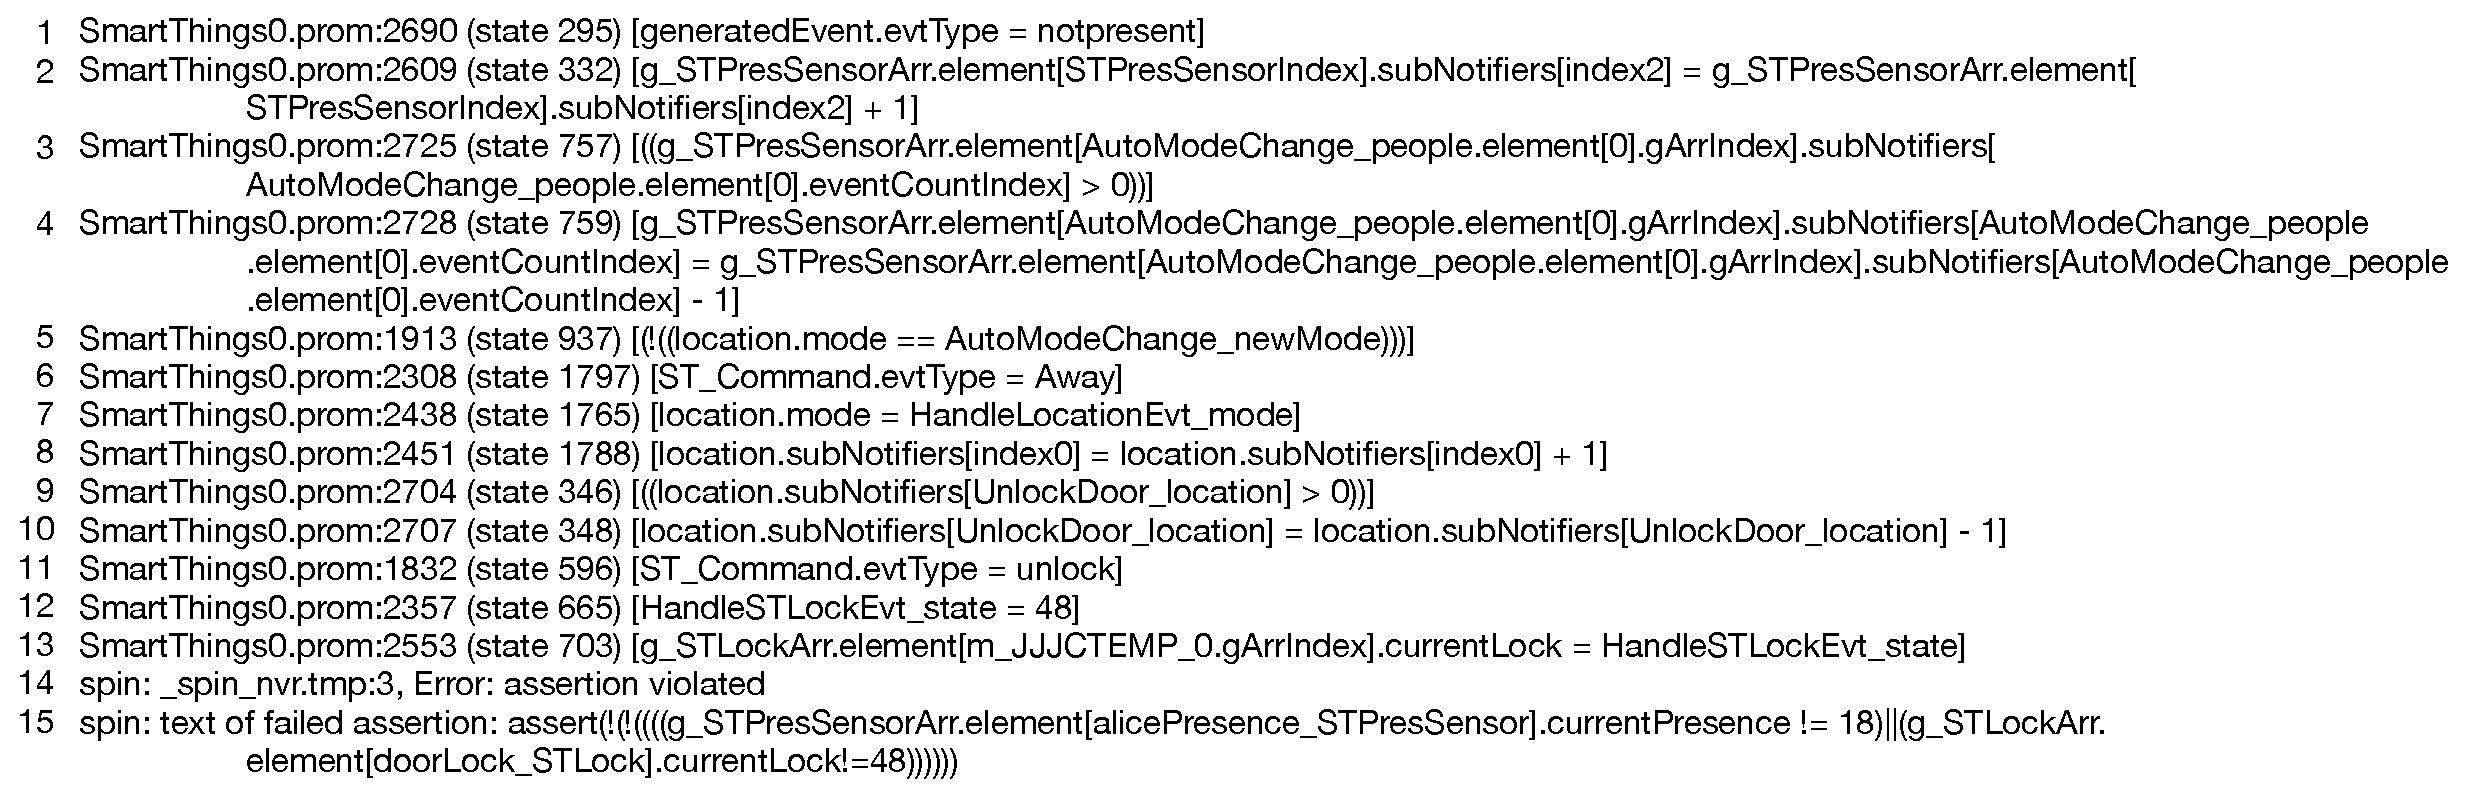
\includegraphics[width=6.1in]{verificationlog}
	%\mbox{\lstinputlisting[language=groovy]{./code/violationlog.cc}}
	%\parbox[6.0in]{\lstinputlisting[language=groovy]{./code/violationlog.cc}}
	%\lstinputlisting[language=groovy]{./code/violationlog.cc}
	%\vspace{-0.17in}
    \caption{Example violation log (filtered).}
	\label{verificationlog}
\end{center}
%\vspace{-0.2in}
\end{figure}


Figure~\ref{verificationlog} shows the (filtered) violation log (a counter-example) output by \spin.
The format of each line in the violation log is as follows:
file name (\textit{SmartThings0.prom}), line number, state number, and the executed code.
In particular, the counter example has the following steps.
{\bf (1)} The event \textit{not present} is generated by \texttt{Alice's presence} if Alice leaves home (line 1)
and its subscribers are notified of this state change (line 2).
{\bf (2)} The app \textit{Auto Mode Change} reads and processes this state change event (lines 3-5)
and notifies the location manager to change the location mode to \textit{Away} (line 6).
{\bf (3)} The location manager changes its mode and notifies its subscribers of this change (lines 7-8).
{\bf (4)} The app \textit{Unlock Door} reads and processes this mode change event (lines 9-10)
and sends an $unlock$ command to the device \texttt{Door Lock} (line 11),
which unlocks the door (lines 12-13).
Thus, the system enters an unsafe physical state (\ie, the main door is unlocked when no one is at home) (lines 14-15).

Upon closer inspection, the description of \textit{Unlock Door} suggests
that it unlocks the door {\em only upon user input}.
However, in practice, it also unlocks the door whenever the location mode changes
(\ie, there is an inconsistency between the app's description and its implementation).
